% Drawing 138/06-50 -- folder 138, batch 06, archive page 119 (PDF page 120).
% Transcription: un tripode avec un sommet sur une branche, $1$ ; une boucle avec une queue, marquée d'une croix ; des esquisses encadrées de traits et en partie biffées, $1$, $\mathbb{Z}_2$ ; un tripode suivi d'un segment à sommet, marqué $*$, $\mathbb{Z}_2$ ; un cercle avec une queue à deux sommets, $\mathbb{Z}_2$.
% Kind: table of small maps with automorphism groups (f). Method 2 (schematic redraw from the facsimile). Status: partial.
% Notes: f): a tripod with a vertex on one branch, 1 (circled, with a star); a loop with a tail, drawn over a cross; sketches framed by long strokes and partly struck, 1 and Z_2 (the sketches inside the frame are a reading); a tripod followed by a segment with a vertex, marked *, Z_2; a circle with a tail carrying two vertices, Z_2. The ink stains at the right of the page are not drawings. Each small map carries its automorphism group as written (given as labels, since the transcription names them); vertex positions and loop shapes approximate.
% Coordinates: 1 unit = 1 mm = 1/100 of the crop width (bbox in page fractions: [0.097, 0.113, 0.584, 0.303]).
% Redrawn by Claude (claude-opus-5-5), issue #73, 2026-11-07; not checked by a human; not compiled (no TeX in the session).
% Rights: reproduces part of the work -- behind RENDER_TRANSCRIPTS, never published by itself.
\documentclass[tikz,border=3pt]{standalone}
\usepackage{amsmath,amssymb}
\usetikzlibrary{patterns,arrows.meta}
\tikzset{pencil/.style={black!45}, struck/.style={black!35}, mark/.style={circle,draw,inner sep=1.3pt}, pt/.style={circle,fill,inner sep=0.9pt}, opt/.style={circle,draw,fill=white,inner sep=1.1pt}}
\begin{document}
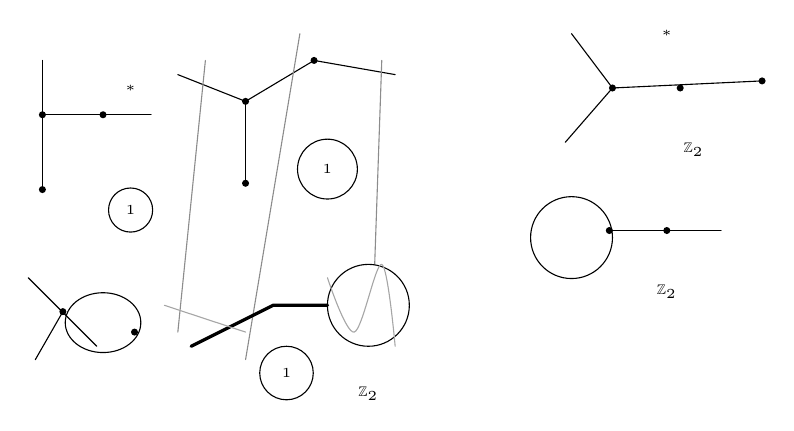
\begin{tikzpicture}[x=1mm,y=1mm,line cap=round,line join=round,font=\scriptsize]
\draw (5.2,-10.3) -- (5.2,-26.7);
\draw (5.2,-17.2) -- (19,-17.2);
\node[pt] at (5.2,-17.2) {};
\node[pt] at (5.2,-26.7) {};
\node[pt] at (12.9,-17.2) {};
\node[inner sep=1pt] at (16.4,-13.8) {\tiny $*$};
\draw (16.4,-29.3) circle[radius=2.8];
\node[inner sep=1pt] at (16.4,-29.3) {\tiny $1$};
\draw (3.4,-37.9) -- (12.1,-46.6);
\draw (4.3,-48.3) -- (7.8,-42.2);
\draw (12.9,-43.6) ellipse[x radius=4.8, y radius=3.8];
\node[pt] at (7.8,-42.2) {};
\node[pt] at (16.9,-44.8) {};
\draw (31,-15.5) -- (22.4,-12.1);
\draw (31,-15.5) -- (39.7,-10.3);
\draw (31,-15.5) -- (31,-25.9);
\node[pt] at (31,-15.5) {};
\node[pt] at (31,-25.9) {};
\node[pt] at (39.7,-10.3) {};
\draw (39.7,-10.3) -- (50,-12.1);
\draw[pencil] (25.9,-10.3) -- (22.4,-44.8);
\draw[pencil] (37.9,-6.9) -- (31,-48.3);
\draw[pencil] (48.3,-10.3) -- (47.4,-36.2);
\draw[very thick] (24.1,-46.6) -- (34.5,-41.4) -- (41.4,-41.4);
\draw (46.6,-41.4) ellipse[x radius=5.2, y radius=5.2];
\draw[struck] (20.7,-41.4) -- (31,-44.8);
\draw[struck] plot[smooth, tension=0.55] coordinates {(41.4,-37.9) (44.8,-44.8) (48.3,-36.2) (50,-46.6)};
\draw (41.4,-24.1) circle[radius=3.8];
\node[inner sep=1pt] at (41.4,-24.1) {\tiny $1$};
\draw (36.2,-50) circle[radius=3.4];
\node[inner sep=1pt] at (36.2,-50) {\tiny $1$};
\node[inner sep=1pt] at (46.6,-52.6) {\tiny $\mathbb{Z}_2$};
\draw (77.6,-13.8) -- (72.4,-6.9);
\draw (77.6,-13.8) -- (71.6,-20.7);
\draw (77.6,-13.8) -- (96.6,-12.9);
\node[pt] at (77.6,-13.8) {};
\node[pt] at (86.2,-13.8) {};
\node[pt] at (96.6,-12.9) {};
\node[inner sep=1pt] at (84.5,-6.9) {\tiny $*$};
\node[inner sep=1pt] at (87.9,-21.6) {\tiny $\mathbb{Z}_2$};
\draw (72.4,-32.8) circle[radius=5.2];
\draw (77.2,-31.9) -- (91.4,-31.9);
\node[pt] at (77.2,-31.9) {};
\node[pt] at (84.5,-31.9) {};
\node[inner sep=1pt] at (84.5,-39.7) {\tiny $\mathbb{Z}_2$};
\end{tikzpicture}
\end{document}
